\newpage 

\subsection{Building Electrical Channels: Transistors}

\noindent
To even begin to manage currents and voltages, we will need a way to control the flow of electricity:

\begin{Def}[Transistor]

    A \textbf{transistor} is a small electronic semiconductor device. A \textbf{semiconductor} (e.g., silicon) is a material with electrical 
    conductivity between that of a \textbf{conductor} (well at conducting electricity) and an \textbf{insulator}
    (not conducting electricity). It has two main functions:
    \begin{itemize}
        \item \textbf{Switching:} Transistors can act as electronic switches, turning current on or off.
        \item \textbf{Amplification:} Transistors can amplify weak electrical signals, making them stronger.
    \end{itemize}

    \noindent
    These devices can easily heat up, so for lower current applications, transistors are encased in resin/plastic,
    while in higher current applications, they have a side made with metal to dissipate heat. These resistors
    are often attached to a \textbf{heat sink}, which is a piece of metal that draws heat away from the transistor.\\
    \noindent
    \rule{\textwidth}{0.4pt}\\

    \noindent
    A transistor has three terminals (pins) made of silicon or germanium:
    \begin{itemize}
        \item \textbf{Emitter (E):} The terminal through which current flows out of the transistor.
        \item \textbf{Base (B):} The terminal that controls the transistor's operation.
        \item \textbf{Collector (C):} The terminal through which current flows into the transistor.
    \end{itemize}
    \medskip
    \noindent
    These may be in different order depending on the make and model. A \textbf{part number} is often printed on the front, which may be 
    used to look up the manufacturer's \textbf{datasheet} (specifications of the transistor).
\end{Def}

\begin{figure}[ht!]
    \centering
    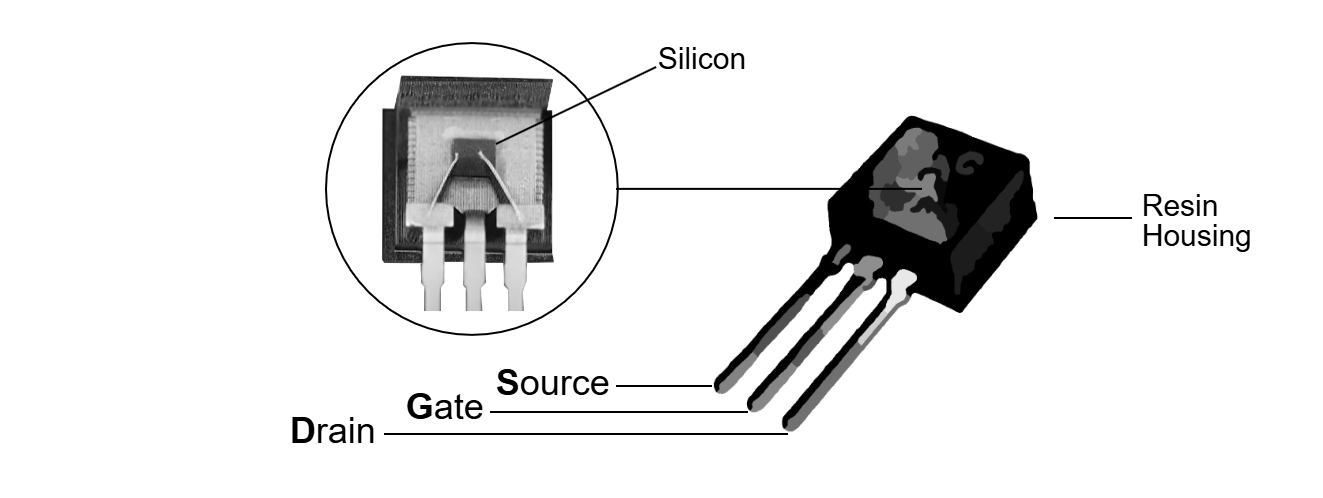
\includegraphics[width=1\textwidth]{Sections/circuits/transistor.png}

    \vspace{1em}
    \caption{A transistor with its three terminals: Emitter (E), Base (B), and Collector (C), all of which are 
    composed of silicon, while the inner workings are encased in resin.}
    \label{fig:transistor}
\end{figure}